\section{Punto de Vista de Realización de Requerimientos}
El punto de vista de realización de requerimientos se basa en las necesidades que se requieren subsanar y que el sistema debe cumplir de manera satisfactoria, estos requerimientos, son los que definen las funciones que el sistema será capaz de realizar, describiendo las transformaciones que el sistema realiza sobre las entradas para producir salidas. Por decirlo de otra manera, estos requerimientos son los que posteriormente se van a transformar en algoritmos, es decir, en las funcionalidades del sistema.
Para la obtención de estos requerimientos, es necesario ademas de cumplir a detalle con una serie de pasos específicos, tener los objetivos, los cuales son el punto de partida para los requerimientos. Esta serie de pasos son: obtención, análisis, especificación, verificación y aceptación. Luego de esto, en la realización de requerimientos es en donde se especializan estos requerimientos.


\subsection{Modelo de Realización de Requerimientos}
\begin{figure}[h!]
	\centering
	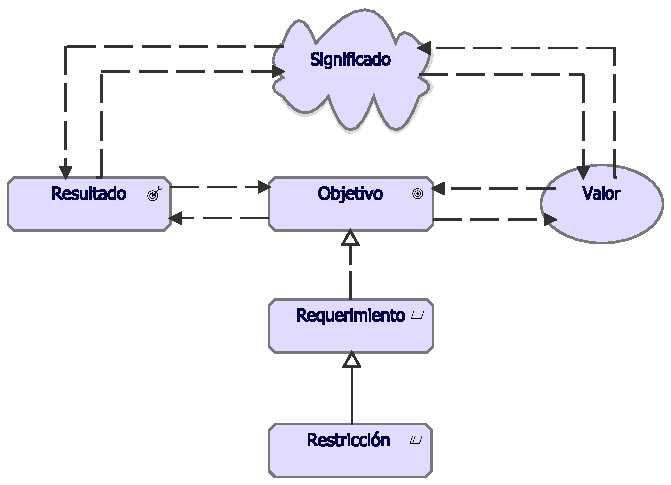
\includegraphics[width=1.0\linewidth]{imgs/modelo/RealRequerimientos}
	\caption{Modelo Realización de Requerimientos}
\end{figure}

El modelo del punto de vista de realización de requerimientos, como se ha evidenciado en los anteriores puntos de vista, parte de un objetivo central, del cual todo se desglosa, cuenta con diversas partes y herramientas como lo es el significado, valor, resultado y finalmente un requerimiento el cual se puede especializar cuantas veces lo permita.

%\newpage

\subsection{Caso  de Contribución de Objetivos}
\begin{figure}[h!]
	\centering
	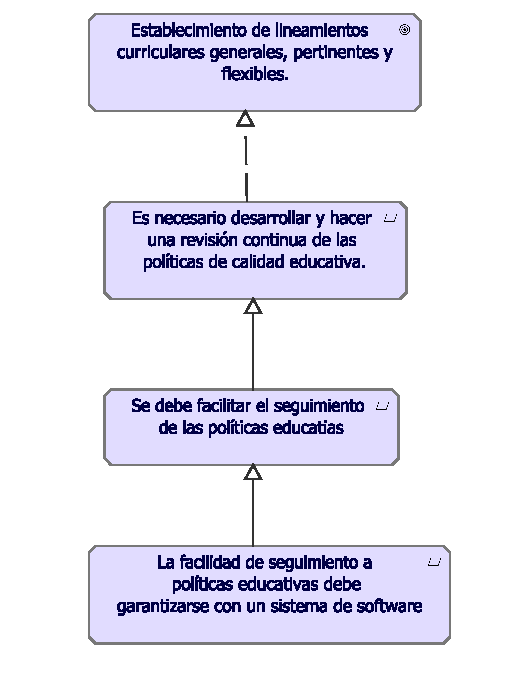
\includegraphics[width=1.0\linewidth]{imgs/motivacion/RealizaRequerimientos/realizaRequerimientos.pdf}
	\caption{Caso Realización de Requerimientos}
\end{figure}

En el proyecto planteado con el ministerio de educación nacional (MEN), y para la construcción del punto de vista de realización de requerimientos, en primer lugar se escogió un objetivo central del proyecto el cual es, Establecimiento de lineamientos curriculares generales, pertinentes y flexibles. A partir de este objetivo central, se dedujo un requerimiento como lo es: es necesario desarrollar y hacer una revisión continua de las políticas de calidad educativa, requerimiento del cual se puede especializar, tal como se hizo con el proyecto: se debe facilitar el seguimiento de las políticas educativas, y a su vez, esta especialización de requerimiento se pudo especializar una vez más: la facilidad de seguimiento a políticas educativas debe garantizarse con un sistema de software. Esta especialización de los requerimientos en la realización de los mismos, se puede hacer tantas veces como el mismo requerimiento lo permita.